\chapter{Nuestra propuesta}
\label{sec:algoritmo}
\section{Agregando probabilidades a un algoritmo existente}

En esta secci\'on se presenta una modificaci\'on del algoritmo
de~\cite{arec2:2008:Areces} donde el orden fijo de las propiedades de
la escena de entrada se sustituye por una distribuci\'on de probabilidad finita. \\

%Los cambios requeridos son bastante sencillos (v\'ease
%Figuras~\ref{algo:bisim-l} y~\ref{algo:bisim-add-el-over}), pero el comportamiento del algoritmo 
%resultante cambia notablemente. 

Con los cambios propuestos el nuevo algoritmo tiene 3 caracter\'isticas nuevas:
\begin{itemize}
 \item Es no determin\'istico: dos ejecusiones del algoritmo con la
misma entrada podr\'{i}an resultar en diferentes REs para los objetos en la escena.\\

 \item Conseguimos mayor sobreespecificaci\'on: simulando lo que encontramos en el corpus.\\

 \item Podemos generar una distribuci\'on de probabilidad
para las ER generadas por el algoritmo si lo ejecutamos muchas veces con
el mismo input. Como vamos a mostrar emp\'{i}ricamente en
Secci\'on~\ref{sec:evaluacion}, dado un corpus de ER para una escena determinada,
es posible calcular una distribuci\'on de probabilidad adecuada para la
probabilidad de uso de las propiedades y relaciones en la escena, de tal manera que
la distribuci\'on de probabilidad de las ER generadas para el modelo
simule la que se encuentra en el corpus.\\
\end{itemize}

En las siguientes secciones explicaremos el input y output del algoritmo, luego el algoritmo en detalle, como conseguimos asegurar terminaci\'on, como se generan las ER no-determin\'isticamente, como conseguimos mayor sobreespecificaci\'on y luego veremos como calcular las \puse\ que el algoritmo toma como input para ambos casos, cuando tenemos un corpus disponible para la escena y target y cuando no lo tenemos, para finalizar daremos un ejemplo de ejecuci\'on.

\section{Input/Output del algoritmo}
\label{input_algo}
El sistema toma como input el contexto tambi\'en llamado modelo y una lista de probabilidades de las propiedades y relaciones de la signatura del modelo.

El contexto lo toma en un archivo XML codificado de la siguiente manera: tanto las relaciones como propiedades aparecen como relaciones, pero en el caso de las propiedades se van a relacionar con un elemento adicional ficticio agregado al contexto, por ejemplo, que codifica el hecho de que $e_1$ es \emph{amarillo} diciendo que est\'a relacionado con ese elemento ficticio por la relaci\'on binaria \emph{amarillo}. 

Las relaciones ternarias o de mayor orden se pueden codificar como relaciones binarias de la siguiente manera, con una relaci\'on a cada elemento que forme parte de la relaci\'on. 


\begin{verbatim}
<?xml version="1.0"?>
<problem id="e1">
  <individual id="e1">
    <related rel="pequeno" to="c" />
    <related rel="amarillo" to="c" />
    <related rel="esfera" to="c" />
  </individual>
  <individual id="e2">
    <related rel="cubo" to="c" />
    <related rel="rojo" to="c" />
    <related rel="pequeno" to="c" />
    <related rel="abajo-de" to="e3" />
  </individual>
  <individual id="e3">
    <related rel="esfera" to="c" />
    <related rel="amarillo" to="c" />
    <related rel="pequeno" to="c" />
    <related rel="arriba-de" to="e2" />
  </individual>
  <individual id="e4">
    <related rel="cubo" to="c" />
    <related rel="rojo" to="c" />
    <related rel="grande" to="c" />
    <related rel="a-la-izq-de" to="e5" />
  </individual>
  <individual refer-to="e5">
    <related rel="grande" to="c"/>
    <related rel="esfera" to="c" />
    <related rel="rojo" to="c" />
    <related rel="a-la-der-de" to="e4" />
  </individual>
  <individual id="e6">
    <related rel="pequeno" to="c" />
    <related rel="cubo" to="c" />
    <related rel="amarillo" to="c" />
    <related rel="a-la-izq-de" to="e7" />
  </individual>
  <individual id="e7">
    <related rel="pequeno" to="c" />
    <related rel="cubo" to="c" />
    <related rel="rojo" to="c" />
    <related rel="a-la-der-de" to="e6" />
  </individual>
  <individual id="c">
    <related rel="terminal" to="c" />
  </individual> 
</problem>
\end{verbatim}

La lista de probabilidades Rs, es una lista de pares de tuplas (R, R.\puse) que vinculan a cada
relaci\'on R a una cierta probabilidad de uso R.\puse ordenada de mayor a menor con el orden de preferencia de las propiedades y relaciones. Por ejemplo esta es una lista de probabilidades de uso de la Figura \ref{GRE3D7-stimulus}

esfera 1.0, \\
cubo 1.0,\\
rojo 0.978,\\ 
grande 0.257,\\ 
arriba-de 0.178,\\ 
amarillo 0.15,\\
peque\~no 0.107,\\ 
izquierda 0.007,\\
arriba 0.007, \\
derecha 0, \\
a-la-izq-de 0, \\
a-la-der-de 0, \\
debajo-de 0\\

Es decir, si $\REL$ es el
conjunto de todos los s\'imbolos de relaci\'on en el modelo (es decir, la~\emph{signatura} del modelo), recordemos que tomamos las unarias como relaciones, entonces podemos decir que Rs $\in (\REL \times [0,1])^*$

En la Secci\'on \ref{sec:learning} explicaremos de donde sacar estas probabilidades que el algoritmo toma como input.

Luego de terminar, el algoritmo calcula lo que se llaman las $\mathcal {L}$-clases (clases de la l\'ogica $\mathcal {L}$) de semejanza del modelo de entrada de~$\gM $. Intuitivamente, si dos elementos en el modelo pertenecen a la misma $\mathcal {L}$-clase de similitud, entonces~$\mathcal {L}$ no es lo suficientemente expresiva para diferenciarlos (es decir, no hay una f\'ormula en~$\mathcal {L }$ que pueda distinguirlos).\\

La salida del algoritmo es un conjunto de f\'ormulas (que ser\'an expresiones referenciales si la clase de la f\'ormula contiene s\'olo 1 objeto) de los elementos del modelo. Si cada f\'ormula tiene un solo objeto, tenemos una ER para cada elemento del modelo, es decir el algoritmo da ER para todos los objetos que puede identificar un\'ivocamente. Lo llamaremos $RE$.\\
%Usaremos el contexto \ref{grafo-GRE3D7-stimulus} como ejemplo para mostrar los pasos a seguir para la ejecuci\'on del algoritmo.

%It is clear that a scene can be encoded in different ways as a relational model (for example, we could argue that $e_1$ is also \emph{leftof} $e_2$, and so on).  The algorithm assumes that these issues have been resolved and that the model encodes a suitable representation of the scene we want to describe.  Moreover, we will assume that all relations are \emph{binary}.  We will not consider relations of arity greater than two (relations of higher arity can be encoded as binary relations via reification, if necessary), and unary
%properties can be encoded as binary relations including one additional `dummy' element in the model (e.g., we encode the fact that $e_1$ is \emph{blue} saying that it is related to the dummy element by the \emph{blue} binary relation).

%On termination, the algorithm computes what are called the $\mathcal{L}$-similarity classes of the input model $\gM$. Intuitively, if two elements in the model belong to the same $\mathcal{L}$-similarity class, then $\mathcal{L}$ is not expressive enough to tell them appart (i.e, no formula in $\mathcal{L}$ can distinguish them). 

%In what follows, we will use formulas of the $\el$ description logic language~\cite{baad:desc03} to describe refinement classes.  As discussed in~\cite{arec2:2008:Areces}, this language is suitable for conjunctive relational RE, which are the ones we will find in the corpora used for our evaluation\footnote{Notice, though, that the particular formal language used is independent of the main algorithm, and different add$_{\mathcal{L}}$(R,$\varphi$,\RE) functions can be used depending on the language involved.}. For a detail description of $\el$, we refer to~\cite{baad:desc03}.  For this paper, we only need to know that the interpretation of the formula $\psi \sqcap \exists$R.$\varphi$ is the set of all elements that satisfy $\psi$ and that are related by relation R to some element that satisfy $\varphi$. For example, the interpretation of the formula \emph{esfera} $\sqcap \exists$\emph{leftof}.\emph{cubo} is the set of all esferas that are on the left of some cubo.  

%We are now ready to describe Algorithms~\ref{algo:bisim-l}
%and~\ref{algo:bisim-add-el}. Algorithm~\ref{algo:bisim-l} takes as
%input a model $\gM$ and a list Rs of pairs (R,R.\puse) that links each
%relation R to some probability of use R.\puse. I.e., if $\REL$ is the
%set of all relation symbols in the model (i.e., the \emph{signature}
%of the model) then Rs $\in (\REL \times [0,1])^*$. Moreover, we assume
%Rs to be ordered by R.\puse.



\section{El nuevo algoritmo}

Antes de empezar explicando el algoritmo, daremos algunos conceptos necesarios para entenderlo.

Desde ahora hablaremos de {\it f\'ormulas} (una f\'ormula corresponde a una descripci\'on) por ejemplo usaremos la f\'ormula ``esfera'' para referirnos a todas las esferas del contexto, en el contexto \ref{grafo-GRE3D7-stimulus} ser\'ian: $e_1$, $e_3$ y $e_5$  as\'i como ``esfera y amarillo'' ser\'ian: $e_1$ y $e_3$.\\

Una clase es un conjunto de objetos que satisface la misma f\'ormula (descripci\'on), por ejemplo ``esfera'' ser\'an todas las esferas del modelo.\\

Una f\'ormula es {\it Informativa} cuando tiene m\'as informaci\'on que las f\'ormulas que hay hasta el momento, es decir, la clase de la f\'ormula esta inclu\'ida en alguna otra f\'ormula y no es igual. Por ejemplo si tenemos las f\'ormulas ``esfera'' y ``cubo'' y queremos saber si ``esfera roja'' es informativa, si lo es, ya que $e_5$ es una ``esfera roja'' y existen otras que no son rojas, es decir divide el conjunto de esferas, por lo tanto si lo es. \\

Una f\'ormula es {\it subsumida} si ya tenemos subf\'ormulas con m\'as informaci\'on que cubren todo el conjunto de objetos que la f\'ormula cubr\'ia. Por ejemplo, T que es la f\'ormula en la cual todos los objetos pertenecen, ser\'a subsumida cuando se agreguen las f\'ormulas ``esfera'' y ``cubo'' ya que todos los elementos del contexto \ref{grafo-GRE3D7-stimulus} son o esferas o cubos, es decir ya tenemos informaci\'on m\'as precisa de los objetos.\\

{\it Redundante} es una f\'ormula para la cual ya hay otra f\'ormula la cual tenga los mismos objetos del modelo. Por ejemplo para el contexto \ref{grafo-GRE3D7-stimulus} si ya tenemos la f\'ormula ``esfera roja'', la f\'ormula ``esfera roja grande'' es redundante ya que no agrega informaci\'on porque el conjunto de objetos esferas rojas es solamente 1 objeto.\\

{\it Trivial} es una f\'ormula para la cual no hay objetos que la satisfagan en el modelo considerado, por ejemplo en el Contexto \ref{grafo-GRE3D7-stimulus} ``esfera amarilla grande'' es trivial ya que no hay esferas amarillas grandes en el contexto considerado.\\

Vamos a utilizar f\'ormulas de el lenguaje de descripci\'on $\el$ de la l\'ogica~\cite{baad:desc03} para describir clases de refinamiento \footnote {Note, sin embargo, que el lenguaje formal utilizado en particular es independiente del algoritmo principal, y diferentes funciones add$_{\mathcal {L}}$(R,$\varphi $, \RE) se pueden utilizar en funci\'on del lenguaje en cuesti\'on.}.\\
%Para una descripci\'on detallada de $\el$, nos referimos a~\cite{baad:desc03}.
La {\it interpretaci\'on} de la f\'ormula de $\el$  $\psi \sqcap \exists $R.$ \varphi$ es el conjunto de todos los elementos que satisfagan~$\psi$ y que est\'an relacionados por relaci\'on R con alg\'un elemento que satisface $\varphi $.
Por ejemplo, la interpretaci\'on de la f\'ormula \emph{esfera}$\sqcap$ \emph{a-la-izq-de}. \emph{cubo} es el conjunto de todas las esferas que est\'an a la izquierda de alg\'un cubo.\\


\begin{figure}[!t]
\small
\centering
\begin{algorithm}[H]
\dontprintsemicolon
\caption{Computando clases de $\mathcal{L}$-similaridad}\label{algo:bisim-l}
\KwIn{\footnotesize Un modelo $\gM$ y una lista Rs $\in (\REL \times [0,1])^*$
 de relaciones con sus valores de \puse\, odenados por \puse}
\KwOut{\footnotesize Un conjunto de f\'ormulas \RE tal que
$\{\interp{\varphi} \mid \varphi \in \RE\}$ es el conjunto de clases de
$\mathcal{L}$-similaridad de $\gM$}

$\RE \leftarrow \{\top\}$\tcp*[f]{\footnotesize descripci\'on m\'as general $\top$ aplica a todos los elementos del contexto}

\For{\em (R,R.\puse) $\in$ Rs}{
	R.\randomuse = Random(0,1)\tcp*[f]{\footnotesize R.\randomuse es la probabilidad de usar R} \;
        R.\incuse = (1 $-$ R.\puse) / MaxIterations\tcp*[f]{\footnotesize R.\puse\ incrementadas por R.\incuse en cada ciclo}
}

\Repeat{\em $\forall$((R,R.\puse) $\in$ Rs).(R.\puse $\ge$ 1)\tcp*[f]{\footnotesize R.\puse\ incrementadas hasta que alcanzan 1}}{
  \While(\tcp*[f]{\footnotesize mientras alguna clase tenga al menos 2 elementos}){\em $\exists (\varphi \in$ \RE)$.(\#\interp{\varphi}>1)$}{
      \RE' $\leftarrow$ \RE \tcp*[f]{\footnotesize hacer una copia para futura comparaci\'on} \;
      \For{\em (R, R.\puse) $\in$ Rs}{
          \If(\tcp*[f]{\footnotesize R ser\'a usada en la expresi\'on}){\em R.\randomuse $\le$ R.\puse}{
              \lFor{\em $\varphi \in$ \RE}{
                  add$_\mathcal{EL}$(R, $\varphi$, \RE)\tcp*[f]{\footnotesize refine todas las clases usando R}}
                  }\;
              \If(\tcp*[f]{\footnotesize la clasificaci\'on cambi\'o}){\em \RE $\not =$ \RE'}{exit\tcp*[f]{\footnotesize salga del ciclo for para tratar de nuevo con la m\'as alta R.\puse}}
              }
     \If(\tcp*[f]{\footnotesize la clasificaci\'on se ha estabilizado}){\em \RE $=$ \RE'}{exit\tcp*[f]{\footnotesize salga del ciclo while para incrementar R.\puse}}
  }
  \lFor{\em (R,R.\puse) $\in$ Rs}{
    R.\puse $\leftarrow$ R.\puse $+$ R.\incuse\tcp*[f]{\footnotesize incrementar R.\puse}
  }
}
\end{algorithm}

\begin{algorithm}[H]
\dontprintsemicolon
\caption{add$_\el$(R, $\varphi$, \RE)} \label{algo:bisim-add-el-over}

\If(\tcp*[f]{\footnotesize primera iteraci\'on?}){\em FirstLoop?}{
    Informativa $\leftarrow$ TRUE \tcp*[f]{\footnotesize permitir sobreespecificaci\'on}}
\lElse(\tcp*[f]{\footnotesize informativa: tiene menos objetos que la original?}) {Informativa $\leftarrow$ $\interp{\psi \sqcap \exists \mbox{\em R}.\varphi} \neq \interp{\psi}$} 
\For{\em $\psi \in$ \RE con $\#\interp{\psi} > 1$}{
  \If{\em $\psi \sqcap \exists$R.$\varphi$ no esta subsumida en \RE\ {\bf y} \tcp*[f]{\footnotesize no-redundante: no puede ser obtenida desde \RE?}\\
    \em \ \ \ $\interp{\psi \sqcap \exists \mbox{\em R}.\varphi} \neq \emptyset$ {\bf y} \tcp*[f]{\footnotesize es no-trivial: tiene elementos?}\\
     \ \ \  \emph{Informativa}}{
    y $\psi \sqcap \exists \mbox{R}.\varphi$ to $\RE$ \tcp*[f]{\footnotesize agregar la nueva clase a la clasificaci\'on} \;
    borrar f\'ormulas subsumidas de $\RE$ \tcp*[f]{\footnotesize borrar clases redundantes}
  }
}
\end{algorithm}
\vspace*{-.5cm}\caption{Algoritmos de refinamiento con probabilidades y sobreespecificaci\'on para el \el-language}\label{fig:algo3}

\end{figure}


%Tenemos 2 algoritmos~\ref{algo:bisim-l} y~\ref{algo:bisim-add-el-over}. 

%El algoritmo~\ref{algo:bisim-l} toma como entrada un modelo $\gM$ y una lista de pares de tuplas (R, R.\puse) que vinculan a cada
%relaci\'on R a una cierta probabilidad de uso R.\puse (nombrada en \ref{input_algo}). 
%Es decir, si $\REL$ es el
%conjunto de todos los s\'imbolos de relaci\'on en el modelo (es decir, la~\emph{signatura} del modelo), recordemos que tomamos las unarias como relaciones, entonces R $\in (\REL \times [0,1])^*$. Por otra parte, asumimos que R esta ordenada por R.\puse\ de mayor a menor.
%\textcolor{blue}{deberia reemplazar aca que R es un conjunto por una lista ordenada...}

%\begin{figure}[t]
%\peque\~no
%\centering
%\begin{algorithm}[H]
%\dontprintsemicolon
%\caption{Computing $\mathcal{L}$-similarity classes}\label{algo:bisim-l}
%\KwIn{\footnotesize A model $\gM$ and a list Rs $\in (\REL \times [0,1])^*$
 %of relation symbols with their \puse\ values, ordered by \puse}
%\KwOut{\footnotesize A set of formulas \RE such that
%$\{\interp{\varphi} \mid \varphi \in \RE\}$ is the set of
%$\mathcal{L}$-similarity classes of $\gM$}
%
%$\RE \leftarrow \{\top\}$\tcp*[f]{\footnotesize the most general description $\top$ applies to all elements in the scene}
%
%\For{\em (R,R.\puse) $\in$ Rs}{
	%R.\randomuse = Random(0,1)\tcp*[f]{\footnotesize R.\randomuse is the probability of using R} \;
        %R.\incuse = (1 $-$ R.\puse) / MaxIterations\tcp*[f]{\footnotesize R.\puse\ are incremented by R.\incuse in each loop}
%}
%
%\Repeat{\em $\forall$((R,R.\puse) $\in$ Rs).(R.\puse $\ge$ 1)\tcp*[f]{\footnotesize R.\puse\ are incremented until they reach 1}}{
  %\While(\tcp*[f]{\footnotesize while some class has at least two elements}){\em $\exists (\varphi \in$ \RE)$.(|\interp{\varphi}|>1)$}{
      %\RE' $\leftarrow$ \RE \tcp*[f]{\footnotesize make a copy for future comparison} \;
      %\For{\em (R, R.\puse) $\in$ Rs}{
          %\If(\tcp*[f]{\footnotesize R will be used in the expression}){\em R.\randomuse $\le$ R.\puse}{
              %\For{\em $\varphi \in$ \RE}{
                  %add$_\mathcal{L}$(R, $\varphi$, \RE)\tcp*[f]{\footnotesize refine all classes using R}}
                  %}\;
              %\If(\tcp*[f]{\footnotesize the classification has changed}){\em \RE $\not =$ \RE'}{exit\tcp*[f]{\footnotesize exit for-loop to try again highest R.\puse}}
              %}
     %\If(\tcp*[f]{\footnotesize the classification has stabilized}){\em \RE $=$ \RE'}{exit\tcp*[f]{\footnotesize exit while-loop to increase R.\puse}}
  %}
  %\For{\em (R,R.\puse) $\in$ Rs}{
    %R.\puse $\leftarrow$ R.\puse $+$ R.\incuse\tcp*[f]{\footnotesize increase R.\puse}
  %}
%}
%\end{algorithm}
%\vspace*{-.5cm}\caption{Main algorithm, dealing with probabilities}\label{fig:algo1}
%\end{figure}
%
%
%\begin{figure}[t]
%\peque\~no
%\centering
%\begin{algorithm}[H]
%\dontprintsemicolon
%\caption{add$_\el$(R, $\varphi$, \RE)} \label{algo:bisim-add-el}
%
%\For{\em $\psi \in$ \RE with $|\interp{\psi}| > 1$}{
  %\If(\tcp*[f]{\footnotesize informative:peque\~noer than the original?}){\em $\psi \sqcap \exists$R.$\varphi$ is not subsumed in \RE\ {\bf and} \tcp*[f]{\footnotesize non-redundant:can't be obtained from \RE?}\\
    %\em \ \ \ $\interp{\psi \sqcap \exists \mbox{\em R}.\varphi} \neq \emptyset$ {\bf and} \tcp*[f]{\footnotesize non-trivial:has elements?}\\
     %\ \ \ $\interp{\psi \sqcap \exists \mbox{\em R}.\varphi} \neq \interp{\psi}$ }{
    %add $\psi \sqcap \exists \mbox{R}.\varphi$ to $\RE$ \tcp*[f]{\footnotesize add the new class to the classification} \;
    %remove subsumed formulas from $\RE$ \tcp*[f]{\footnotesize remove redundant classes}
  %}
%}
%\end{algorithm}
%\vspace*{-.5cm}\caption{Refinement function for the \el-language}\label{fig:algo2}
%\end{figure}

%The set $\RE$ will contain the formal description of the refinement
%classes and it is initialized by the most general description $\top$.
%For each R, we first compute R.\randomuse, a random number in [0,1].
%If R.\randomuse $\le$ R.\puse\ then we will use R to refine the set of
%classes.  The value of R.\puse\ will be incremented by $R.\incuse$ in
%each main loop, to ensure that all relations are, at some point,
%considered by the algorithm.  This ensures that a referring expression
%will be found if it exist; but gives higher probability to expressions
%using relations with a high R.\puse.
% 
%While $\RE$ contains descriptions that can be refined (i.e., classes
%with at least two elements) we will call the refinement function
%add$_\mathcal{L}$(R,$\varphi$,$\RE$) successively with each relation
%in Rs. A change in one of the classes, can trigger changes in
%others. For that reason, if $\RE$ changes, we exit the for-loop to
%start again with the relations of higher R.\puse. If the after trying
%to refine the set with all relations in Rs, the set $\RE$ has not
%changed, the we have reach a stable state (i.e., the classes described
%in $\RE$ cannot be further refined, using the current R.\puse\
%values). We will then increment all the R.\puse\ values and start the
%procedure again.

%Algorithm~\ref{algo:bisim-add-el} coincides with the one described
%in~\cite{arec2:2008:Areces}.  It will refine each of the descriptions
%in $\RE$ using the relation R and the other descriptions already in
%$\RE$, under certain conditions. The new description should be
%\emph{non-redundant} (the new class cannot be obtained as the union of
%classes already represented in $\RE$), \emph{non-trivial} (the new
%class is not empty), and \emph{informative} (the new class should not
%coincide with the original class).  If all this conditions are met,
%the new description is added to $\RE$, and redundant descriptions
%possible created by the addition of the new description are
%eliminated.

%Suppose fixed an input model $\gM$ and values for Rs, and fix also
%some target element $t$.  Assume also that $t$ indeed has an
%$\el$-referring expression.  Upon termination,
%Algorithm~\ref{fig:algo1} will compute an $\el$ formula $\varphi$ such
%that $\interp{\varphi} = \{t\}$, but $\varphi$ might be different in
%each run of the algorithm (even though $\gM$ and Rs are fixed).  If we
%repeat this experiment a statistically significant number of times, we
%can define an estimate of the probability distribution of the REs
%generated by the algorithm for $t$, given $\gM$ and Rs. In
%Section~\ref{sec:evaluation} we will show that given a corpus of REs
%for $\gM$, it is possible to define R.\puse\ values so that this
%probability distribution matches with good accuracy the probability
%distribution of REs found in the corpus.


El conjunto $\RE$ contendr\'a la descripci\'on formal de las clases de refinamiento
y es inicializado por la descripci\'on m\'as general $\top$.\\

Recorremos Rs, para cada R (relaciones de la signatura del dominio REL), primero calculamos R.\randomuse, un n\'umero aleatorio en [0,1], y R.incuse que ser\'a (1 -R.puse) / MaxIterations, siendo MaxIterations el n\'umero m\'aximo de iteraciones del ciclo principal que queremos permitir.\\

Si R.\randomuse $\le$ R.\puse\ entonces vamos a utilizar R para refinar el conjunto de
clases. \\

El valor de R.\puse\ se incrementar\'a en $R.\incuse$
en cada ciclo principal, para asegurar que todas las relaciones son en alg\'un momento,
consideradas por el algoritmo. Esto asegura que una expresi\'on referencial
se encontrar\'a si existe; pero dar\'a mayor probabilidad a las expresiones
que usan las relaciones con m\'as alta R.\puse.\\
 
Mientras que $\RE$ contiene descripciones que pueden ser refinadas (es decir, clases
con al menos dos elementos) vamos a llamar a la funci\'on de refinamiento
add$_\mathcal{EL}$(R,$\varphi$,$\RE$) sucesivamente con cada relaci\'on
de Rs.\\

 Un cambio en una de las clases, puede desencadenar cambios en
las otras. Por esa raz\'on, si $\RE$ cambia, salimos del ciclo for y volvemos a
empezar con las relaciones de m\'as alta R.\puse. \\

%Si despu\'es de probar refinar el conjunto con todas las relaciones de Rs, el conjunto $\RE$ no ha
%cambiado, hemos alcanzado un estado estable (es decir, las clases que se describen
%en $\RE$ no puede ser refinadas, utilizando los valores de R.\puse\). 
%A continuaci\'on, se incrementar\'an todos los valores de R.\puse\ y se iniciar\'a el
%procedimiento de nuevo.\\
%El algoritmo~\ref{algo:bisim-add-el-over} coincide con el descripto
%en~\cite{arec2:2008:Areces}. 
Se refinar\'a cada una de las descripciones
en $\RE$ utilizando la relaci\'on R y las otras descripciones que ya est\'an en
$\RE$, bajo ciertas condiciones. \\

La nueva descripci\'on debe ser
\emph{no redundante} (la nueva clase no se puede obtener como la uni\'on de
clases ya representadas en $\RE$), \emph{no trivial} (la nueva
clase no es vac\'{i}a), es \emph{informativa} (la nueva clase no debe
coincidir con la clase original). Si se cumplen todas estas condiciones,
la nueva descripci\'on se a\~nade a $\RE$, y las descripciones redundantes
posiblemente creadas por la adici\'on de la nueva descripci\'on son
eliminadas.\\

%Supongamos que se fija un modelo de entrada $\gM$ y los valores de Rs (R.\puse \ para todos los elementos de la signatura del modelo), y se fija tambi\'en alg\'un elemento target $t$. Supongamos tambi\'en que $t$ tiene una expresi\'on referencial en 
%$\el$. Cuando termine el
%Algoritmo~\ref{algo:bisim-l} habr\'a calculado una f\'ormula $\varphi$ de $\el$ tal
%que $\interp{\varphi} = \{t\}$, pero $\varphi$ pueden ser diferentes en
%cada ejecuci\'on del algoritmo (a pesar de que $\gM$ y Rs son fijos). \\
%
%Si repetimos este procedimiento un n\'umero estad\'{i}sticamente significativo de veces,
%podemos definir una estimaci\'on de la distribuci\'on de probabilidad de las ER
%generadas por el algoritmo para $t$, dado $\gM$ y Rs. En la
%Secci\'on~\ref{sec:evaluacion} vamos a demostrar que dado un corpus de ER
%para $\gM$, es posible definir los valores de R.\puse\ para que esta
%distribuci\'on de probabilidad coincida con buena precisi\'on a la distribuci\'on de probabilidad de ER que se encuentra en el corpus.


\subsection{Asegurando terminaci\'on}

Uno de los problemas que ten\'ian otros algoritmos es que no siempre terminaban, para asegurar terminaci\'on nosotros incrementamos las probabilidades aleatorias en cada ciclo, hasta que alcancen 1

Definimos MaxIterations como la cantidad m\'axima de iteraciones que vamos a permitir, y calculamos R.incuse es cuanto vamos a incrementar la probabilidad de R en cada ciclo, 

R.incuse = (1 -R.puse) / MaxIterations

con esto nos aseguramos que en MaxIterations todas lleguen a 1, y en consecuencia el algoritmo termine, ya que la l\'inea 15 del c\'odigo, se incrementa R.puse con R.incuse y en la 16 dice salir del ciclo principal si para todas las R, R.puse es >=1

\subsection{Generando ER relacionales}

Nuestro algoritmo permite generar relaciones con otros objetos e incliur las ER de los dem\'as objetos, no tiene preferencia por las relaciones ni por las propiedades proposicionales, en el sentido de que va o no incluirlas de acuerdo a la probabilidad de uso que ellas tengas, las cuales fueron calculadas o sacadas de un corpus.

\subsection{Generando ER no-determin\'isticamente}

Al iniciar el algoritmo (en l\'inea 3) calcula para cada R, R.rnduse que es un n\'umero aleatorio entre 0 y 1, ese n\'umero va a hacer que el algoritmo sea no-determin\'istico, ya que en la l\'inea 9, el algoritmo usar\'a R para refinar las clases solamente si 
R.rnduse >= R.puse. Por lo tanto y considerando que en las siguientes ejecuciones R.rnduse ser\'an distintos, va a poder generar distintas ER.

\subsection{Generando descripciones sobreespecificadas}\label{sec:overspecification}


El algoritmo original~\ref{algo:bisim-l}
 permit\'ia muy poca sobreespecificaci\'on en las ER que
generaba. Una relaci\'on con una baja \puse\ podr\'{i}a ser suficiente
(Por s\'{i} mismo o en combinaci\'on con algunas de las relaciones ya consideradas) para
identificar el target. Una vez que se a\~nadi\'o esa relaci\'on, se obtiene una ER, pero una ER m\'as corta, m\'as espec\'{i}fica podr\'{i}a ser encontrada, mediante la eliminaci\'on de algunos de los refinamientos anteriores.
Por lo tanto, la ER resultante podr\'{i}a ser sobreespecificada. Este es el mismo tipo de sobreespecificaci\'on
que permite el algoritmo incremental. Pero se ha argumentado~\cite{Engelhardt_Bailey_Ferreira_2006, Arts_Maes_Noordman_Jansen_2011} que
un grado mucho mayor de sobreespecificaci\'on se encuentra generalmente en corpora, y esto
es de hecho lo que se ve en el corpus GRE3D7. Como podemos ver en la tabla~\ref{corpus-distribution},
el target es descripto 16,43 \% de las veces como ``peque\~na green ball'' cuando ``green ball'' ya es una ER. Con el uso de los valores de \puse\ aprendidos con el c\'alculo explicado en la secci\'on anterior, el algoritmo original no pueden simular este comportamiento.\\

Debido a que la idea fundamental del algoritmo es la sem\'antica, la manipulaci\'on sobreespecificaci\'on en
una forma natural es dif\'{i}cil de obtener. Si dos propiedades tienen la misma interpretaci\'on en un determinado
modelo, entonces una vez que la primera ha sido considerada, la segunda no refinar\'a las clases
obtenidas hasta el momento, y por lo tanto, el algoritmo no la incluir\'a en las descripciones generadas.
Por otro lado, si hacemos caso omiso de la condici\'on de la restricci\'on de informatividad (es decir,
el hecho de que la adici\'on de una relaci\'on debe refinar la clase, eliminando algunos de
los elementos que contiene), entonces corremos el riesgo de generar descripciones como ``bola verde verde''.\\

--No me gusta esta parte--
Como soluci\'on de compromiso, consideramos la siguiente variaci\'on del algoritmo
original %~\ref{algo:bisim-l} 
hacemos caso omiso de la restricci\'on de informatividad (es decir, que permite la inclusi\'on de nuevas relaciones
en la descripci\'on, incluso si no refinan la clase asociada) \emph{pero s\'olo durante el
primer bucle del algoritmo}. Es decir, durante el primer bucle sobre los elementos de la
lista de probabilidades Rs, se permitir\'a la inclusi\'on de todas las relaciones que no trivializan la
descripci\'on (es decir, la clase asociada no est\'a vac\'{i}a). Debido a que esto se hace s\'olo durante
el primer bucle, sabemos que las propiedades repetidas no aparecer\'an en las ER generadas.
En los bucles restantes, se a\~nadir\'an propiedades adicionales s\'olo si son de car\'acter informativo.\\

\subsection{Generando ER para plurales}

Este algoritmo devuelve ER para todos los elementos del contexto, 
esto implica que podr\'iamos dar expressiones referenciales de un conjunto de elementos.

Por ejemplo queremos identificar a $e_1$ y $e_5$ 
siendo resultados dados por el algoritmo que $e_1$
esfera, amarillo, peque\~no
y $e_5$ esfera, rojo


En la siguiente secci\'on explicaremos como calcular R.\puse\ cuando tenemos corpus disponible, y cuando no lo tenemos.

\section{Obteniendo probabilidades de uso}

%\subsection{Aprendizaje autom\'atico desde un corpus para describir nuevos objetos}
\label{sec:learning}

En la secci\'on anterior hemos presentado un algoritmo que supone que para
cada relaci\'on R se tiene una conocida
probabilidad de uso R.\puse. En esta secci\'on, se describe c\'omo
calcular estas probabilidades a partir de corpus. Asumimos disponible un corpus de ER asociada a diferentes
escenas t\'{i}picas del dominio en el que el algoritmo GER tiene que operar. Mostramos primero c\'omo calcular los valores de R.\puse\ para
esas escenas para las que se dispone de un corpus de ER. A continuaci\'on, mostramos c\'omo
generalizar estos valores a otras escenas en el dominio, utilizando un
algoritmo de aprendizaje autom\'atico. En primer lugar vamos a ejemplificar la
metodolog\'{i}a utilizando el corpus GRE3D7 que introducimos en ~\ref{sec:corpusGRE} y, a continuaci\'on mostraremos c\'omo hacer lo mismo con el corpus TUNA introducido en~\ref{sec:corpusTUNA}.


\subsection{Calculando \puse\ cuando hay disponible un corpus para la escena considerada}

Las Figuras \ref{rojo-amarillo} y  \ref{verde-azul} son las escenas del corpus GRE3D7 introducido en \ref{sec:corpusGRE}, est\'an agrupadas seg\'un los colores que tienen.\\

\begin{figure}
\centering
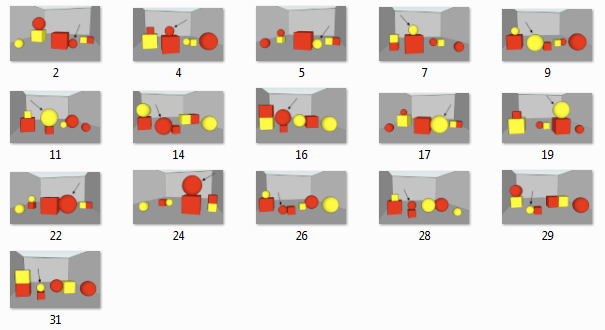
\includegraphics[width=1\textwidth]{images/rojo-amarillo.png}
\caption{Im\'agenes del GRE3D7 parte rojo y amarillo}
\label{rojo-amarillo}
\end{figure}

\begin{figure}
\centering
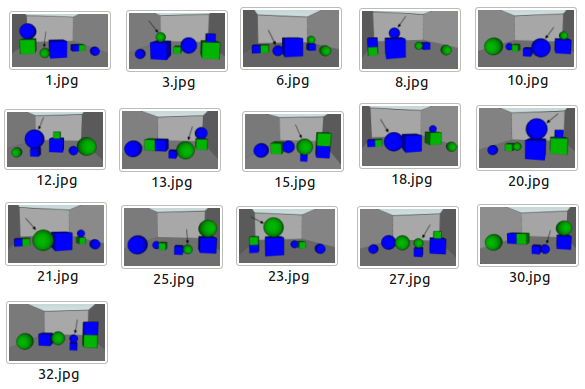
\includegraphics[width=1\textwidth]{images/imagenesML.png}
\caption{Im\'agenes del GRE3D7 parte azul y verde}
\label{verde-azul}
\end{figure}


\begin{figure}[ht]
\begin{minipage}[b]{0.5\linewidth}
\centering
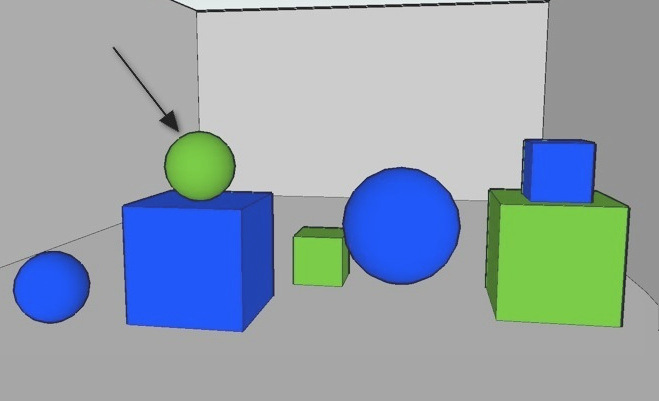
\includegraphics[width=\textwidth]{images/3.jpg}
%\vspace*{1cm}
\caption{Contexto 3 del GRE3D7}
\label{fig3}
\end{minipage}
\hspace*{1cm}
\begin{minipage}[b]{0.5\linewidth}
%\centering
%\begin{figure}[ht]
%\begin{center}
green ball \\
small green ball  \\
small green ball on-top red large cube \\
green ball on-top blue cube\\
green ball on-top large blue cube \\
small green ball on-top blue cube  \\
ball on-top cube \\
small green ball on-top red large left cube  \\
small ball on-top cube large  \\
top green ball   \\
green ball on-top cube  \\
\caption{ER dadas por personas para el Contexto \ref{fig3}}
\label{ER-fig3}
\end{minipage}
\end{figure}


El corpus tiene para cada imagen 140 ER dadas por personas. Las ER dadas en \ref{ER-fig3} son las ER diferentes que aparecieron en el corpus para el Contexto \ref{fig3}, pero... uno se imagina un corpus en que las personas usaron distintas palabras para nombrar lo mismo, distintas frases, distinto orden de las palabras, s\'i es verdad, este corpus ya est\'a limpio de todas esas cosas, pero si quisieramos partir de un corpus con las ER tal cual dieron las personas, tendr\'iamos que realizar los siguientes pasos a fin de unificar el vocabulario:

\begin{enumerate}
\item Tokenizar las expresiones referenciales y llamar al conjunto de palabras distintas
 $Pal$. En particular, las expresiones de varias palabras como ``arriba de'', ``encima de''
  debe ser igualadas a una \'unica palabra que signifique lo mismo, digamos \emph{arriba-de}.

\item Eliminar hiper\'onimos de $Pal$. Por ejemplo, si ambos \emph{cubo} y
  \emph{cosa} aparecen en $Pal$ para nombrar la misma cosa, eliminar \emph{cosa}, ya que \emph{cubo} es m\'as espec\'ifico.

\item Si el conjunto de palabras obtenidas en los pasos anteriores contiene
  sin\'onimos normalizarlos con un representante de la clase.  Por ejemplo, las palabras \emph{chico}
  y \emph{peque\~no} son ambas representadas por la palabra \emph{peque\~no}.

\item Llamar al conjunto resultante $\REL$; que ser\'a la signatura del modelo $\gM$ utilizada por el algoritmo.

\item Para cada escena, definir $\gM$ tal que la interpretaci\'on
 $\interp {\cdot}$ asegure de que todas las ERs encontradas en el corpus sean ER en
  el modelo. Por ejemplo, las %$\el$ f\'ormulas correspondientes%
	ER de \ref{ER-fig3} deben denotar el target se\~nalado en la Figura \ref{fig3} el modelo 
$\gM$ est\'a representado en Figura~\ref{modelo-fig3}.
%GRE3D7-stimulus-cap2
\item Para cada R$\in \REL$ calculo R.\puse \ utilizando~(\ref{eq1}) si
  hay muchas ER para cada escena (caso corpus GRE3D7) o asignamos 1 a R.\puse \ si R esta en ER, asignamos 0 en caso contrario (caso corpus TUNA).
\end{enumerate}

En el caso del GRE3D7 ya estaba unificado el vocabulario y la signatura del modelo es 
$\REL = \{green, ball, small, ontop, red, large, cube, blue, left, top\} $

\begin{figure}[ht]
\centering
\begin{tikzpicture}
  [
    n/.style={circle,fill,draw,inner sep=3pt,node distance=1.4cm},
    aArrow/.style={->, >=stealth, semithick, shorten <= 2pt, shorten >= 2pt},
  ]
 \node[n,label=above:$e_1$,label=below:{
    \relsize{-1}$\begin{array}{c}
      \nLeft\\[-2pt]
      \nSmall\\[-2pt] 
      \nBlue \ \  
      \nBall\end{array}$}] (a) {};

 \node[n,label=above:$e_2$,label=below:{
    \relsize{-1}$\begin{array}{c}
      \nLeft\\[-2pt]
      \nBig\\[-2pt] 
      \nBlue \ \  
      \nCube\end{array}$}, right of=a] (b) {};

 \node[n,label=below:$e_3$,label=above:{
    \relsize{-1}$\begin{array}{c}
      \nTop \ \       \nLeft \ \ 
      \nSmall \ \       \nGreen \ \ 
      \nBall\end{array}$}, above of=b] (c) {};

 \node[n,label=above:$e_4$,label=below:{
    \relsize{-1}$\begin{array}{c}
      \nSmall\\[-2pt] 
      \nGreen\\[-2pt] 
      \nCube\end{array}$}, right of=b] (d) {};

 \node[n,label=above:$e_5$,label=below:{
    \relsize{-1}$\begin{array}{c}
      \nBig\\[-2pt] 
      \nBlue\\[-2pt] 
      \nBall\end{array}$}, right of=d] (e) {};

 \node[n,label=above:$e_6$,label=below:{
    \relsize{-1}$\begin{array}{c}
      \nBig\\[-2pt] 
      \nGreen\\[-2pt] 
      \nCube\end{array}$}, right of=e] (f) {};

 \node[n,label=below:$e_7$,label=above:{
    \relsize{-1}$\begin{array}{c}
      \nTop \ \ 
      \nSmall\ \ 
      \nBlue \ \  
      \nCube\end{array}$}, above of=f] (g) {};

 \draw [aArrow,bend right=90] (b) to node[auto,swap]{\relsize{-1}$\nBelow$} (c);
 \draw [aArrow,bend right=90] (c) to node[auto,swap]{\relsize{-1}$\nOntop$} (b);

 \draw [aArrow,bend right=30] (d) to node[auto,swap]{\relsize{-1}$\nLeftof$} (e);
 \draw [aArrow,bend right=30] (e) to node[auto,swap]{\relsize{-1}$\nRightof$} (d);

 \draw [aArrow,bend right=90] (f) to node[auto,swap]{\relsize{-1}$\nBelow$} (g);
 \draw [aArrow,bend right=90] (g) to node[auto,swap]{\relsize{-1}$\nOntop$} (f);

 \draw[dotted] (-.65,-1.2) rectangle (7.1,2.1);

 \end{tikzpicture}
\vspace*{-.4cm}\caption{El modelo del Contexto \ref{fig3}}
\label{modelo-fig3}
\end{figure}

La regresi\'on lineal es un m\'etodo matem\'atico que modela la relaci\'on que hay entre una variable dependiente Y, las variables independientes Xi y un t\'ermino aleatorio E.  \\

Vamos a tomar la parte \ref{verde-azul} del corpus GRE3D7 para aprender las probabilidades de uso de cada palabra en las ER que di\'o la gente, y as\'i darnos una idea de como es la distribuci\'on del uso de las palabras del conjunto $REL$ en el corpus.\\

Vamos a usar las siguientes propiedades, las cuales las sacamos autom\'aticamente del XML del corpus.

\begin{small}
\begin{table}[h]
\begin{center}
\begin{tabular}{|l|p{10cm}|}
\hline
target-tiene & cuando el elemento target tiene la propiedad. \\
\#rel-prop & n\'umero de propiedades y relaciones que el target tiene.\\
\#rel & n\'umero de relaciones que el target tiene. \\
landmark-tiene & cuando un landmark del target tiene la propiedad, un objeto es un landmark si tiene una relaci\'on directa en el modelo, con el target (lo usamos para el GRE3D7).\\
location-has & cuando la RE puede usar la ubicaci\'on del target en la figura (esto se hizo porque el TUNA corpus tiene algunas ER donde se le dijo a la gente que pod\'ian usar la localizaci\'on del objeto).\\
discrimination & calculada como 1 sobre el n\'umero de objetos en el modelo que tienen la propiedad.  \\
\hline
\end{tabular}
\caption{Caracter\'isticas usadas para conseguir f\'ormulas con regresi\'on lineal que nos den una idea de la \puse de las palabras} 
\label{features}
\end{center}
\end{table}
\end{small}

\begin{table}[h!]
\begin{center}
\caption{F\'ormulas y errores de regresi\'on lineal para todo el corpus \ref{verde-azul}}
\label{tabla-linear-regresion-all}
\begin{tabular}{|l|c|c|l|}
\hline
Palabra &Error promedio	LR	& Error-PM	& F\'ormula de LR\\
\hline
ball		 &0.0465   &0.0609	  & 0.2894 * disc-gatt + 0.7883\\
\hline
cube		 &0.0417	 &0.0531	  &0.49   * disc-gatt - 0.0129\\
\hline
\hline
blue		 &0.0353	 &0.0454	  &0.848  * target-tiene + 0.1073\\
\hline
green		 &0.0264	 &0.046	    &0.8722 * target-tiene + 0.0016\\
\hline
\hline
large		 &0.1762	 &0.2378	  &0.5911 * target-tiene + 0.0354\\
\hline
small		 &0.1499	 &0.1755	  &0.3918 * target-tiene + 0.2478 * landmark-tiene -\\
				 &				 &					&0.0913\\
\hline
\hline
left-of  &0.0041	 &0.0094	  &0.0131 * target-tiene +\\
				 &				 &					&0.0253 * adj-target-tiene - 0.0507\\
\hline
on-top	 &0.0706	 &0.1594	  &0.2942 * target-tiene \\
\hline
right-of &0.0029	 &0.0049	  &0.0153 * target-tiene + 0.001\\
\hline
\hline
left		 &0.0068	 &0.0101	  &0.0346 * adj-target-tiene - 0.0653\\
\hline
right		 &0.0079	 &0.0092	  &-0.0118 * disc-gatt + 0.0141\\
\hline
front    &0.0099 	 &0.0135		& 0.0069\\
\hline
center	 &0.0023	 &0.0037	  &0.0047 * target-tiene + 0.0047 * adj-target-tiene +\\
				 &				 &					&0.0029 * vecino-tiene - 0.009\\
\hline
\end{tabular}
\end{center}
\end{table}

En la Tabla \ref{tabla-linear-regresion-all} podemos ver por ejemplo que {\it ball} tiene una \puse alta, es natural ya que en el corpus \ref{verde-azul} todos los targets son {\it ball}, en cambio se puede ver que {\it cube} no es tan alta y depende de la discernibilidad, este n\'umero en la \puse debe leerse como la probabilidad de usar {\it cube} en la descripci\'on del landmark. En los casos de {\it blue} y {\it green} el valor de \puse depende de si el target es {\it blue} o {\it green}, entonces si el target es {\it blue}, le da un valor alto a {\it blue} y bajo a {\it green} y viceversa, no depende del valor de discernibilidad en el modelo.
En la tabla tambi\'en podemos ver que relaciones como {\it small} y {\it large} tienen un error mucho mas alto que el resto de las relaciones, esto se debe a que ellas son propiedades vagas... 
Las relaciones {\it ontop}, {\it leftof} y {\it rightof} dependen fuertemente si el target tiene esa relaci\'on y en caso de tenerla igualmente la \puse no es muy alta, esto indica que en un porcentaje del 30\% por ejemplo se usa {it ontop} y en menos del 3\% left-of o rightof, esta observaci\'on fue reportada en (Viethen, 2011)
Una caracter\'istica interesante que se no fue mencionada en trabajo previo es que tama\~no es m\'as frecuente usado para sobreespecificaci\'on cuando el target y el landmark tienen el mismo tama\~no 
(es usado en ER sobreespecificadas el 49\% cuando el target y el landmarck comparten el tama\~no, y s\'olo el 25\% cuando no lo comparten)


Supongamos que queremos generar autom\'aticamente ER para el target $t$ en una
determinada escena, y que tenemos disponible un corpus $C$ de ER de $t$
en esa escena (esto es exactamente el tipo de informaci\'on que encontramos en el
GRE3D7 corpus \textit{y en el TUNA-corpus}). Utilizamos las ER de $C$
para definir el modelo relacional utilizado por el algoritmo. Entonces 
estimaremos el valor de \puse\ para cada una de las relaciones en el modelo como el
porcentaje en que aparece la relaci\'on en las ER. Es decir,
\begin{equation} \label{eq1}
R.\puse = \frac {\#\mbox{de ERs en $C$ en el que aparece R}} {\#\mbox{de las ER en $C$}}.
\end{equation}

En el caso del corpus TUNA el c\'alculo no es necesario
porque tenemos solo una ER para cada escena.

Esta estimaci\'on es demasiado simplificada y, por ejemplo, no 
diferencia las propiedades del target y las propiedades de
los landmarks utilizadas en una ER relacional para completar la descripci\'on
del target. Pero es muy f\'acil de calcular, y vamos a ver
en la Secci\'on~\ref{sec:evaluacion} que ya produce ER naturales
que coinciden con las encontradas en el corpus.


Las ERs, cantidad de ocurrencias y porcentaje del corpus para de la Figura~\ref{GRE3D7-stimulus-cap2} se muestran en la tabla~\ref{corpus-distribution}, la signatura resultante y su asociado \puse\ figuran en las tres primeras columnas de la tabla~\ref{probability-of-use}.\\

ARREGLAR ESTA TABLA HABIA UNO MAL... ver original...
\begin{table}[h!]
\begin{center}
\begin{tabular}{|l|c|c|}
\hline
Expresiones Referenciales & Cantidad de ocurrencias & Porcentage \\
\hline

green ball & 91 & 65.00\% \\
small green ball   & 23 & 16.43\% \\
small green ball on-top red large cube & 8 & 5.71\% \\
green ball on-top blue cube & 5 & 3.57\% \\
green ball on-top large blue cube & 5 & 3.57\% \\
small green ball on-top blue cube & 2 & 1.43\% \\
ball on-top cube & 1 & 0.71\% \\
small green ball on-top red large left cube  & 1 & 0.71\% \\
small ball on-top large cube & 1 & 0.71\% \\
top green ball  & 1 & 0.71\% \\
%peque\~no esfera on-top cube small & 1 & 0.71\% \\
green ball on-top cube & 1 & 0.71\% \\

\hline
\end{tabular}
\caption{Expresiones Referenciales producidas por las personas para la Figura~\ref{GRE3D7-stimulus-cap2}}\label{corpus-distribution}
\end{center}
\end{table}


Observe que los valores R.\puse\ obtenidos de esta manera deben ser
interpretados como la probabilidad de utilizar R para describir el target en
modelo de $\gM $, y podr\'{i}amos argumentar que se correlacionan con la
 prominencia de R en el modelo. Por esa raz\'on, por ejemplo, el
valor de \emph{esfera}.\puse\ es 1, mientras que el valor de
\emph{cubo}.\puse\ es 0.178. \\

Estas probabilidades no ser\'an \'utiles
para describir los diferentes targets en diferentes escenas. Veremos c\'omo se
pueden utilizarlas para obtener valores para los nuevos targets y escenas utilizando un
enfoque de aprendizaje autom\'atico en la siguiente secci\'on. No es de extra\~nar,
que usando estos valores para R.\puse\ las ER generadas con mayor frecuencia por el
algoritmo se puedan encontrar en el corpus. Como discutiremos en la Secci\'on~\ref{sec:evaluacion} el algoritmo genera ER
con una distribuci\'on que coincide con la encontrada en el corpus y, como la
Tabla~\ref{results-algo-fig3} muestra, incluso las ER generadas por el algoritmo que no se encontraron
en el corpus son naturales.





\subsection{Calculando \puse\ para el target para escenas sin corpus } 
\label{subsec:learning}

%If there is no corpora that describes the target we can estimate the
%\puse~from corpora on a different scenes in the same domain.
%
%We use simple features to obtain the function, all the features can be
%extracted automatically from the relational model and are listed in

Si no hay corpus de expresiones referenciales que describen el target, se puede estimar la \puse~a partir de corpus de
diferentes escenas en el mismo dominio.
Usamos caracter\'isticas simples para obtener una funci\'on que nos dar\'a la probabilidad de cada palabra en el nuevo modelo, todas las caracter\'isticas se pueden extraer de forma autom\'atica desde el modelo relacional y se enumeran en la Tabla~\ref{features}.

\begin{small}
\begin{table}[h]
\begin{center}
\begin{tabular}{|l|p{10cm}|}
\hline
target & cuando el elemento target tiene la propiedad. \\
\#rel-prop & n\'umero de propiedades y relaciones que el target tiene.\\
\#rel & n\'umero de relaciones que el target tiene. \\
landmark & cuando un landmark del target tiene la propiedad, un objeto es un landmark si tiene una relaci\'on directa en el modelo, con el target (lo usamos para el GRE3D7).\\
location-has & cuando la RE puede usar la ubicaci\'on del target en la figura (esto se hizo porque el TUNA corpus tiene algunas ER donde se le dijo a la gente que pod\'ian usar la localizaci\'on del objeto).\\
discrimination & calculada como 1 sobre el n\'umero de objetos en el modelo que tienen la propiedad.  \\
\hline
\end{tabular}
\caption{Caracter\'isticas usadas para aprendizaje autom\'atico de las \puse~para cada palabra en la signatura de los modelos de \textit{GRE3D7 y TUNA-corpus} \label{features}}
\end{center}
\end{table}
\end{small}

% The most important characteristic of the GRE3D7 domain is
%that we are not able to learn, and has an impact in our performance,
%the properties of type size (namely, peque\~no and grande) are used much
%more when the target cannot be uniquely identified with taxonomical
%(esfera and cubo) and absolute (green and blue) properties only.  In
%other words, in the GRE3D7 corpus the size is used more often (90.2\%)

En el caso del GRE3D7 usamos la parte verde-azul, es decir todas las im\'agenes que tienen colores verde y azul, para acotar el problema, asumiendo que la otra parte dar\'ia algo similar. En la siguiente figura se muestran los contextos considerados.


Para hacer el aprendizaje, separamos 1 contexto al que llamamos testing, y todos los dem\'as de entrenamiento. Por ejemplo para aprender \puse del contexto 13, se usaron los contextos: 1,3,6,8,10,12,15,18,20,21,23,25,27,30 y 32. Y as\'i sucesivamente para los dem\'as contextos.

Nuestro conjunto de caracter\'{i}sticas es intencionadamente simplista con el fin de que sea
independiente de dominio. Como resultado hay algunas relaciones complejas
entre las caracter\'{i}sticas de las escenas que no es capaz de
capturar. La caracter\'{i}stica m\'as importante del dominio GRE3D7
que no somos capaces de aprender, y tiene un impacto en nuestro desempe\~no, es que
las propiedades de tama\~no (es decir, peque\~no y grande) se utilizan mucho
m\'as cuando el target no puede ser identificado s\'olo con las propiedades taxon\'omicas absolutas 
(verde y azul) y (esfera y cubo). En otras palabras, en el corpus GRE3D7 se utiliza el tama\~no con m\'as frecuencia (90,2 \%)
cuando la ER resultante no es sobreespecificada y cuando si es sobreespecificada el (34 \%). 
Puede que no sea posible aprender esta caracter\'{i}stica de los
datos del GRE3D7 ya que incluso con las funciones que dependen de dominio definidos
en~\cite[Cap\'{i}tulo 6] {viet:gene11}, no pod\'{i}a ser aprendido por \'arboles decisi\'on. 
Como resultado podemos ver en la tabla~\ref{probability-of-use} de la Figura 13, el valor estimado para 
``grande'' no est\'a cerca de la
valor calculado a partir de corpus. \textit{En el caso de la TUNA-corpus
  mostramos que no podemos aprender la dependencia de la dimensi\'on-X y
  dimensi\'on-y, es decir, cuando una persona a\~nade dimensi\'on-x es altamente
  probable que incluya la dimensi\'on-y en su expresi\'on referencial.}


\begin{figure}[ht]
\begin{minipage}[b]{0.5\linewidth}
\centering
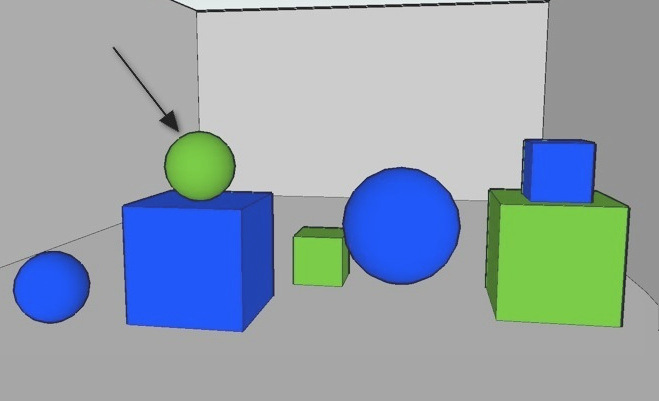
\includegraphics[width=\textwidth]{images/3.jpg}
%\vspace*{1cm}
\caption{Escena 3 del GRE3D7}
\label{GRE3D7-stimulus-3}
\end{minipage}
%\hspace*{-0.35cm}
\begin{minipage}[b]{0.5\linewidth}
\centering
%\begin{figure}[ht]
%\begin{center}
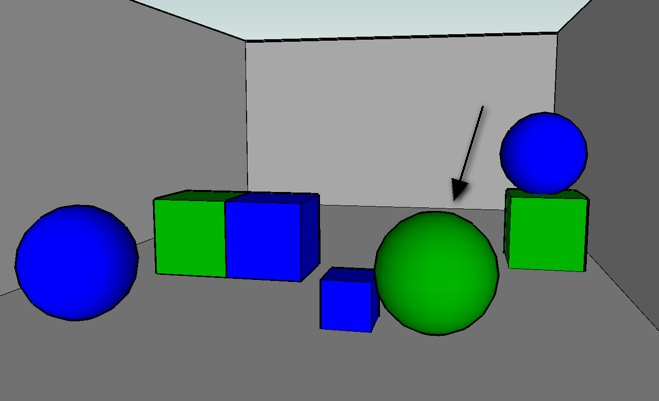
\includegraphics[width=\textwidth]{images/13.jpg}
\caption{Escena 13 del GRE3D7}
\label{GRE3D7-stimulus-13}
\end{minipage}
\end{figure}

\begin{table}[h!]
\begin{center}
\begin{tabular}{|l|c|c|c|c|}
\hline
Palabra &  \puse 					& \puse\ Aprendida & \puse\    							& \puse\  Aprendida \\
        & Modelo \ref{GRE3D7-stimulus-3}   & \ref{GRE3D7-stimulus-3} 				& Modelo \ref{GRE3D7-stimulus-13} 			&  \ref{GRE3D7-stimulus-13}  \\
\hline
esfera & 1.0 & 1.0 & 1.0 & 1.0 \\
cubo & 1.0 & 1.0 & 1.0 & 1.0 \\
verde & 0.978 & 0.993 & 1.0 & 0.9875 \\
peque\~no & 0.257 & 0.346 & 0.0428 & 0.1993 \\
arriba-de & 0.178 & 0.179 & 0 & 0\\ 
azul & 0.15 & 0.124 & 0.064 & 0.1353 \\
grande & 0.107 & 0.03 & 0.307 & 0.7378 \\
izquierda & 0.007 & 0.002 & 0 & 0.0024 \\
arriba & 0.007 & 0 & 0 & 0 \\
derecha & 0 & 0.001 & 0.064 & 0.0005 \\
a-la-izq-de & 0 & 0 & 0 & 0 \\
a-la-der-de & 0 & 0 & 0.064 & 0.1023 \\
debajo-de & 0 & 0 & 0 & 0 \\
\hline
\end{tabular}
\caption{Probabilidades de uso de las palabras del corpus \textit{(GRE3D7) para las Figuras\ref{GRE3D7-stimulus-3} y \ref{GRE3D7-stimulus-13} } 
\label{probability-of-use}}
\end{center}
\end{table}

%The learning was done with the machine learning toolkit
%WEKA~\cite{Hall:WEK09}, training on all minus one (the one for that we
%are learning) for all the scenes of the GRE3D7 \textit{and the
%  TUNA-corpus}.  We use linear regression to learn the function of
%\puse\ for each word in the signature.  For a given scene, we replace
%the variables of the obtained function by the values of the features
%in the scene that we want to describe.

%Using linear regression we are able to learn interesting
%characteristics of the domain. To start with, it learns known facts
%such that the saliency of a color depends strongly on whether the
%target object is of that color, and it does not depend on its
%discrimination power in the model. Moreover, it learns that the on-top
%relation is used more frequently than the horizontal relations
%(left-of and right-of) which confirms a previous finding reported
%in~\cite{viet:gene11}. Finally, it learned a surprising fact of the
%GRE3D7 corpus (not found by previous work), that is that size is used
%more frequently in an overspecified manner when the target and
%landmark share the size. Size was used in overspecified REs in 49\% of
%the descriptions for scenes where target and landmark shared the size,
%and 25\% of the time when target and landmark did not share the
%size. This can be explained by the observation that if landmark and
%target share a property, this property is more salient.

El aprendizaje se realiza con el kit de herramientas de aprendizaje autom\'atico
WEKA~\cite{Hall:WEK09}, entrenando con todas las escenas menos una (para la que estamos aprendiendo) para todas las escenas del \textit{GRE3D7 y TUNA-corpus}. \\
Ejemplo de xml \ref{archivos-xml-tuna}. Notar que no teniamos las imagenes, armamos algunas necesarias nomas, pero no sabemos la unicaci\'on exacta de los objetos.\\

Un ejemplo de archivo de los que toma WEKA como input es para la propiedad blue de la parte muebles del corpus TUNA es \ref{archivos-arff-blue}. 
No recuerdo si esto lo usamos al final o no...
\ref{probabilidad-GATT} , \ref{algoritmo-GATT} 

Utilizamos regresi\'on lineal para aprender la funci\'on de
\puse\ para cada palabra en la signatura. Para una escena determinada, reemplazamos
las variables de la funci\'on obtenida por los valores de las caracter\'{i}sticas
de la escena que queremos describir.\\

Con regresi\'on lineal podemos aprender caracter\'{i}sticas interesantes
 del dominio. Para empezar, se aprenden hechos conocidos
como que color aparezca en la ER depende en gran medida de si el
target es de ese color, y que no depende de su
poder de discriminaci\'on en el modelo. Por otra parte, vimos que la relaci\'on arriba-de
 se utiliza con m\'as frecuencia que las relaciones horizontales
(izquierda y derecha) lo que confirma un hallazgo previo informado
en~\cite{viet:gene11}. Por \'ultimo, vimos en el
GRE3D7 corpus (que no fue reportado por el trabajo anterior), se utiliza el tama\~no
m\'as frecuentemente de una manera sobreespecificada cuando el
target y el landmark comparten el tama\~no. El tama\~no fue utilizado en ER de manera sobreespecificada en el 49 \% de
las descripciones de escenas en las que el target y el landmark compart\'ian el tama\~no,
y el 25 \% cuando target y el landmark no lo compart\'ian. Esto puede explicarse por la observaci\'on de que si landmark y el target comparten una propiedad, esta propiedad es m\'as relevante.



%\section{Aprendizaje autom\E1tico}

%\section{Agregando sobreespecificaci\F3n}
\section{Ejemplo de ejecuci\'on}


En el comienzo ER=$\{\top\}$ y $\interp{\top}$ = $\{e_1, e_2, e_3, e_4, e_5, e_6, e_7\}$ como se puede ver en la Figura~\ref{fig-modelo}.\\


\begin{figure}[ht]
\begin{minipage}[b]{0.45\linewidth}
\centering
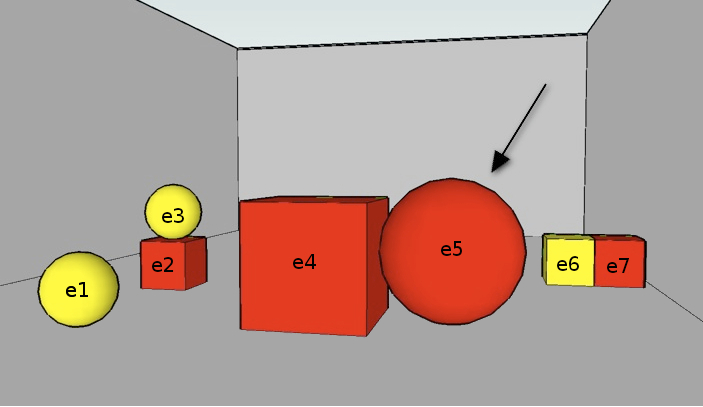
\includegraphics[width=\textwidth]{images/22.jpg}
\vspace*{1cm}
%\caption{Input scene}
\label{GRE3D7-stimulus-22}
\end{minipage}
%\hspace*{-0.35cm}
\begin{minipage}[b]{0.6\linewidth}
\centering
%\begin{figure}[ht]
%\begin{center}
\frame{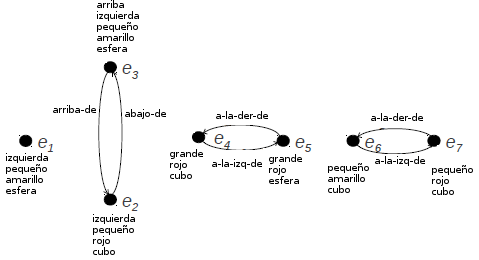
\includegraphics[width=8cm]{images/base.png}}\\[0pt]
\caption{Modelo de la Figura \ref{GRE3D7-stimulus-22}}
\label{fig-modelo}
\end{minipage}
\end{figure}
%El primer bucle del algoritmo es en las propiedades. Para cada propiedad hace add$_\el$ ($\varphi$, RE), las propiedades at\'omicas se muestran en la Figura~\ref{fig-modelo2}.

\begin{figure}[ht]
\begin{center}
\frame{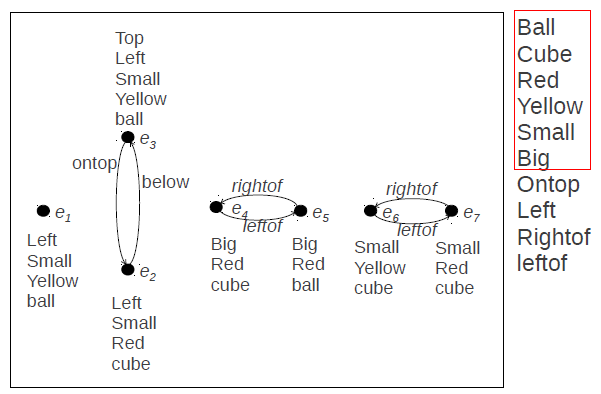
\includegraphics[width=8cm]{images/modelo2.png}}\\[0pt]
\caption{Propiedades proposicionales en cuadro rojo, las del primer ciclo del algoritmo}
\label{fig-modelo2}
\end{center}
\end{figure}

%La primer relaci\'on a considerar es 'esfera', 
%
%La f\'ormula $\varphi$ se a\~nadir\'a a ER si su interpretaci\'on tiene al menos un elemento, a continuaci\'on, para cada f\'ormula
 %$\psi$ en ER la conjunci\'on
%$\varphi  \wedge \psi$ no necesita estar subsumida in ER, la $\interp{\varphi \cup \psi}$ no tiene que ser vac\'io, y su interpretaci\'on tiene que ser distinta de $\interp{\psi}$. Luego las f\'ormulas subsumidas se borran.

La primer relaci\'on a considerar es \textsf{esfera}, recordemos que la f\'ormula $\varphi$ se a\~nadir\'a a ER si su interpretaci\'on tiene al menos un elemento, $\interp{\varphi \cup \psi}$ no tiene que ser vac\'io, y su interpretaci\'on tiene que ser distinta de $\interp{\psi}$. 

ER = \{$\top$, \textsf{esfera}\}, se ven los elementos de la f\'ormula ``esfera'' en un recuadro en la Figura~\ref{fig-modelo3}.

\begin{figure}[ht]
\begin{center}
\frame{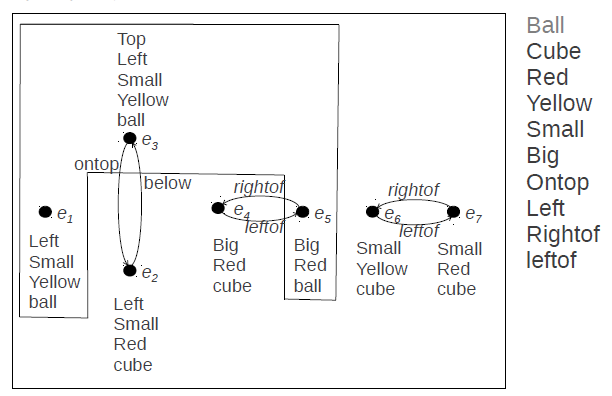
\includegraphics[width=8cm]{images/modelo3.png}}\\[0pt]
\caption{El cuadro indica cuales son ``esfera''}
\label{fig-modelo3}
\end{center}
\end{figure}

La siguiente propiedad es \textsf{cubo}, ER = \{$\top$, \textsf{esfera}, \textsf{cubo}\}, pero ahora la $\interp{\textsf{esfera}}$ = $\{e_1, e_3, e_5\}$, $\interp{\textsf{cubo}}$ = $\{e_2, e_4, e_6, e_7\}$, quedando las particiones como se muestra en la Figura~\ref{fig-modelo4}
\begin{figure}[ht]
\begin{center}
\frame{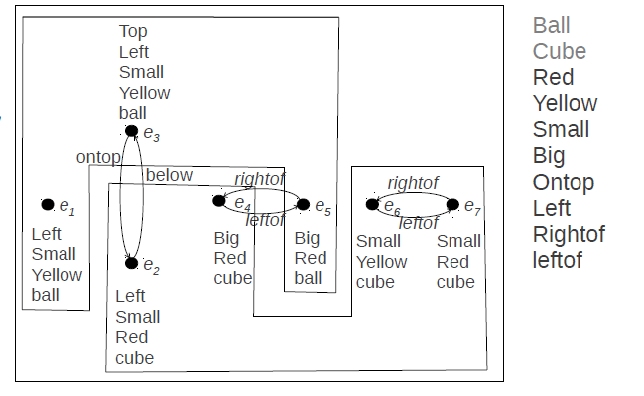
\includegraphics[width=8cm]{images/modelo4.png}}\\[0pt]
\caption{Cuadros indicando ``esfera'' y ``cubo''}
\label{fig-modelo4}
\end{center}
\end{figure}
Ahora podemos borrar $\top$, porque es subsumida (esta cubierta por) las otras dos f\'ormulas. La siguiente propiedad es  \textsf{rojo}, $\interp{\textsf{rojo}}$ es: $\{e_2, e_4, e_5, e_7\}$, haciendo la intersecci\'on con la $\interp{.}$ de cada f\'ormula en ER obtenemos, $\{e_5\}$ y $\{e_2, e_4, e_7\}$, ER = $\{\textsf{esfera}, \textsf{cubo}, \textsf{esfera} \wedge \textsf{rojo}, \textsf{cubo} \wedge \textsf{rojo}\}$, las particiones actuales se pueden ver en la Figura~\ref{fig-modelo9}.
\begin{figure}[ht]
\begin{center}
\frame{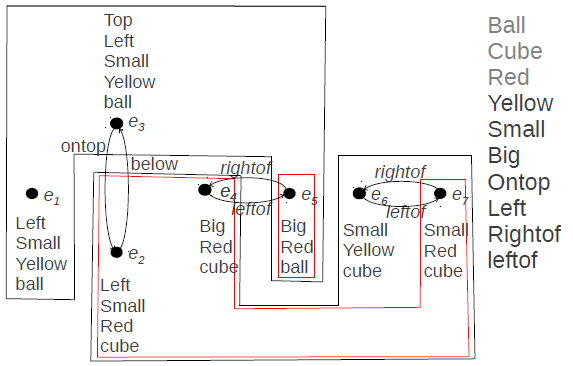
\includegraphics[width=8cm]{images/modelo9.png}}\\[0pt]
\caption{Cuadros indicando ``esfera'', ``cubo'' y ``rojo''}
\label{fig-modelo9}
\end{center}
\end{figure}

Siguiendo con \textsf{amarillo}, tenemos, $\interp{\textsf{amarillo}}$ = $\{e_1, e_3, e_6\}$ y obtenemos ER = $\{\textsf{esfera} \wedge \textsf{amarillo}, \textsf{cubo} \wedge \textsf{amarillo}, \textsf{esfera} \wedge \textsf{rojo}, \textsf{cubo} \wedge \textsf{rojo}\}$. 
Note que aqu\'i ya borramos la f\'ormula \textsf{esfera} porque estaba subsumida, y la f\'ormula \textsf{cubo} tambi\'en. Se muestran particiones en Figura~\ref{fig-modelo10}.

\begin{figure}[ht]
\begin{center}
\frame{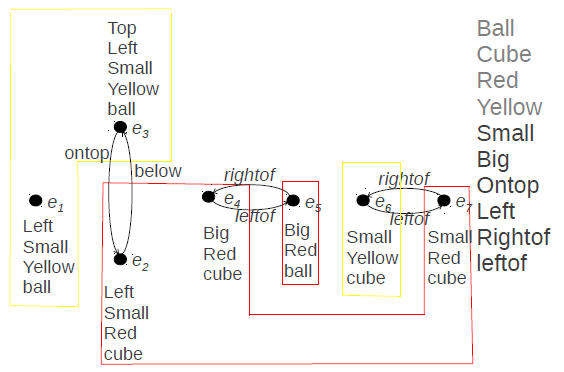
\includegraphics[width=8cm]{images/modelo10.png}}\\[0pt]
\caption{Cuadros indicando ``esfera'', ``cubo'', ``rojo'' y ``amarillo''}
\label{fig-modelo10}
\end{center}
\end{figure}

Haciendo lo mismo con \textsf{peque\~no} tenemos ER = $\{\textsf{esfera} \wedge \textsf{amarillo} \wedge \textsf{peque\~no}, \textsf{cubo} \wedge \textsf{amarillo} \wedge \textsf{peque\~no}, \textsf{esfera} \wedge \textsf{rojo}, \textsf{cubo} \wedge \textsf{rojo}, \textsf{cubo} \wedge \textsf{rojo} \wedge \textsf{peque\~no}\}$, como se puede ver en Figura~\ref{fig-modelo11}.
\begin{figure}[ht]
\begin{center}
\frame{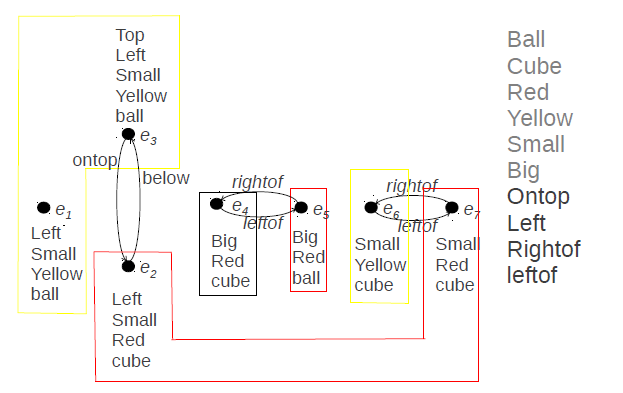
\includegraphics[width=8cm]{images/modelo11.png}}\\[0pt]
\caption{Cuadros indicando ``esfera'', ``cubo'', ``rojo'', ``amarillo'', ``peque\~no'' y ``grande''}
\label{fig-modelo11}
\end{center}
\end{figure}

La siguiente propiedad es \textsf{grande} as\'i, tenemos ER = $\{\textsf{esfera} \wedge \textsf{amarillo} \wedge \textsf{peque\~no}, \textsf{cubo} \wedge \textsf{amarillo} \wedge \textsf{peque\~no}, \textsf{esfera} \wedge \textsf{rojo}, \textsf{cubo} \wedge \textsf{rojo} \wedge \textsf{grande}, \textsf{cubo} \wedge \textsf{rojo} \wedge \textsf{peque\~no}\}$. Aqu\'i no podemos agregar \textsf{grande} a la f\'ormula $\textsf{rojo} \wedge \textsf{cubo}$ porque su interpretaci\'on tiene un solo elemento, y la condici\'on dice que es necesario tener m\'as de uno.

Hasta ahora ER = $\{\textsf{esfera} \wedge \textsf{yellow} \wedge \textsf{peque\~no}, \textsf{cubo} \wedge \textsf{yellow} \wedge \textsf{peque\~no}, \textsf{esfera} \wedge \textsf{rojo}, \textsf{cubo} \wedge \textsf{rojo} \wedge \textsf{grande}, \textsf{cubo} \wedge \textsf{rojo} \wedge \textsf{peque\~no}\}$ 
y tenemos las siguientes extensiones: $\{e_1, e_3\}, \{e_6\}, \{e_5\}, \{e_4\}, \{e_2, e_7\}$ respectivamente. 
Hay dos f\'ormulas que a\'un pueden ser refinadas, $\textsf{esfera} \wedge \textsf{yellow} \wedge \textsf{peque\~no}$ y $\textsf{cubo} \wedge \textsf{rojo} \wedge \textsf{peque\~no}$ 
debido a que tienen m\'as de un elemento cada una, por lo que entran en el ciclo, while del algoritmo 1, en la l\'inea 4. Ahora es el turno de las relaciones, la primera de ellas es \textsf{leftof}, para cada f\'ormula $\varphi$ en ER trataremos de hacer add$_\el$ ($\exists \textsf{leftof}.\varphi$, RE). Notar que $\psi$ solo puede ser $\textsf{esfera} \wedge \textsf{yellow} \wedge \textsf{peque\~no}$ o $\textsf{cubo} \wedge \textsf{rojo} \wedge \textsf{peque\~no}$ porque esos son los que su interpretaci\'on tiene m\'as de un elemento. 
\begin{figure}[ht]
\begin{center}
\frame{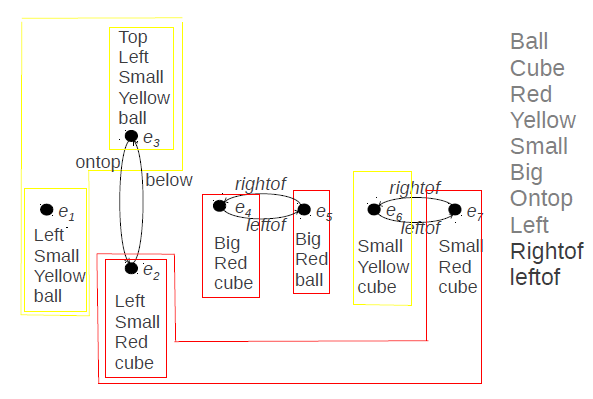
\includegraphics[width=8cm]{images/modelo15.png}}\\[0pt]
\caption{Cuadros indicando ``esfera'', ``cubo'', ``rojo'', ``yellow''...}
\label{fig-modelo15}
\end{center}
\end{figure}


No hay
%because those are the ones that its interpretation have more than one element. There is not 
$\varphi$ y $\psi$ que puedan ser aplicadas. Continuando con \textsf{a-la-der-de} agregamos $\textsf{cubo} \wedge \textsf{yellow} \wedge \textsf{peque\~no} \wedge \exists \textsf{a-la-der-de}. \textsf{cubo} \wedge \textsf{rojo} \wedge \textsf{peque\~no}$, y asi con \textsf{topof} agregamos $\textsf{peque\~no} \wedge \textsf{rojo} \wedge \textsf{cubo} \wedge \exists \textsf{ontop}. \textsf{peque\~no} \wedge \textsf{yellow} \wedge \textsf{esfera}$ y el algoritmo termina con ER = $\{\textsf{esfera} \wedge \textsf{yellow} \wedge \textsf{peque\~no}, \textsf{cubo} \wedge \textsf{yellow} \wedge \textsf{peque\~no}, \textsf{esfera} \wedge \textsf{rojo}, \textsf{cubo} \wedge \textsf{rojo} \wedge \textsf{grande}, \textsf{cubo} \wedge \textsf{rojo} \wedge \textsf{peque\~no}, \textsf{cubo} \wedge \textsf{yellow} \wedge \textsf{peque\~no} \wedge \exists \textsf{a-la-der-de}. \textsf{cubo} \wedge \textsf{rojo} \wedge \textsf{peque\~no}, \textsf{peque\~no} \wedge \textsf{rojo} \wedge \textsf{cubo} \wedge \exists \textsf{ontop}. \textsf{peque\~no} \wedge \textsf{yellow} \wedge \textsf{esfera}\}$, 
aqu\'i todos los elementos est\'an en una clase singleton y no se puede hacer ning\'un refinamiento m\'as. 
%can be applied to $cubo \wedge red \wedge peque\~no$ but there is no formula which interpretation has more than one element to be apply with this one. The same happen for the other relations, so the algorithm ends.
%its interpretation is $\{e_7\}$ with $\psi$ is $cubo \wedge yellow \wedge peque\~no$, the others combinations can't be apply because they don't do true the preconditions. The following relation is rightof, 

%leftof, rightof, ontopof, bellowof

%At this point we already have the target in a singleton set. So the formula for it is ``red and esfera'', and also for s6 which formula is ``yellow cubo''.\\
%As we show this algorithm depends of the order of properties and relations.\\
\begin{figure}[ht]
\begin{center}
\frame{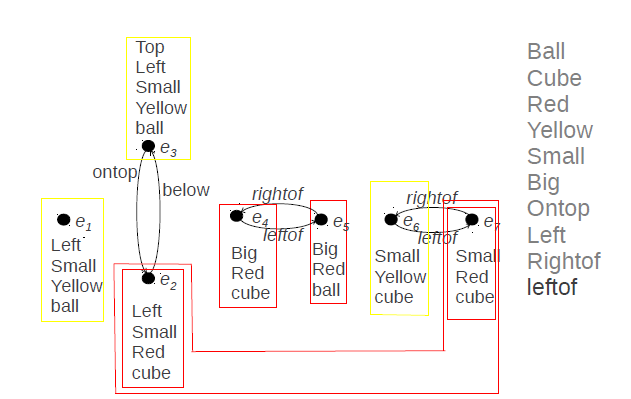
\includegraphics[width=8cm]{images/modelo16.png}}\\[0pt]
\caption{Cuadros indicando ``esfera'', ``cubo'', ``rojo'', ``amarillo''...}
\label{fig-modelo16}
\end{center}
\end{figure}

\begin{figure}[ht]
\begin{center}
\frame{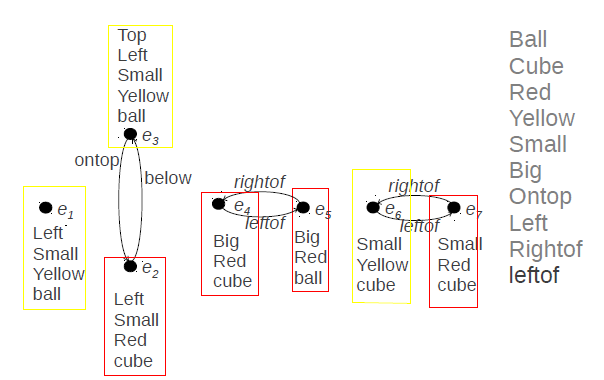
\includegraphics[width=8cm]{images/modelo17.png}}\\[0pt]
\caption{Cuadros indicando ``esfera'', ``cubo'', ``rojo'', ``amarillo''...}
\label{fig-modelo17}
\end{center}
\end{figure}

Las expresiones referenciales encontradas son:\\

$\textsf{esfera} \wedge \textsf{amarillo} \wedge \textsf{peque\~no}$ representa $e_1$ \\
$\textsf{cubo} \wedge \textsf{amarillo} \wedge \textsf{peque\~no}$ representa $e_6$ \\
$\textsf{esfera} \wedge \textsf{rojo}$ representa $e_5$ \\
$\textsf{cubo} \wedge \textsf{rojo} \wedge \textsf{grande}$ representa $e_4$ \\
$\textsf{cubo} \wedge \textsf{rojo} \wedge \textsf{peque\~no}$ representa $\{e_2,e_7\}$  \\
$\textsf{cubo} \wedge \textsf{amarillo} \wedge \textsf{peque\~no} \wedge \exists \textsf{a-la-der-de}. \textsf{cubo} \wedge \textsf{rojo} \wedge \textsf{peque\~no}$ representa $e_6$ \\
$\textsf{peque\~no} \wedge \textsf{rojo} \wedge \textsf{cubo} \wedge \exists \textsf{ontop}. \textsf{peque\~no} \wedge \textsf{amarillo} \wedge \textsf{esfera}$ representa $e_2$ \\

